\documentclass[12pt]{beamer}

\usetheme{Malmoe}
\usepackage[utf8]{inputenc}
\usepackage{graphicx}
\usepackage{xcolor}
\usepackage{wrapfig} % texlive-latex-extra package
\usepackage{underscore}
\usepackage{listings}

\definecolor{Cyan}{RGB}{0,141,184}
\definecolor{codeblock}{RGB}{220,220,220}

\setbeamercolor{structure}{fg=Cyan}

\setbeamerfont{title}{series=\bfseries,parent=structure}
\setbeamerfont{subtitle}{size=\normalsize,series=\bfseries,parent=structure}
\setbeamerfont{author}{size=\scriptsize,series=\bfseries,parent=structure}
\setbeamerfont{institute}{size=\scriptsize,series=\bfseries,parent=structure}
\setbeamerfont{date}{size=\scriptsize,series=\bfseries,parent=structure}

\setbeamerfont{frametitle}{series=\bfseries}

%\ shell code block style (https://en.wikibooks.org/wiki/LaTeX/Source_Code_Listings)
\lstset{language=sh,
	basicstyle=\ttfamily\scriptsize,
	backgroundcolor=\color{codeblock},
	commentstyle=\color{blue},
	breaklines=true,
	breakatwhitespace=true,
	showstringspaces=false
}

\title{GIS.lab}
\subtitle{Fairy Tail About Clever Sysadmin And His Pets}
\author{Ivan Minčík (imincik)}
\setbeamertemplate{navigation symbols}{} 
%\ \institute{}
\date{}
\titlegraphic{
\includegraphics[scale=.1]{images/gislab-logo.png}}


% document BEGIN
\begin{document}


\begin{frame}
	\titlepage
\end{frame}

\begin{frame}[plain]{Once Upon A Time}
	\begin{center}
		
\includegraphics[keepaspectratio=true,width=\textwidth]{images/fairy-tail/dedusko-vecernicek.jpg}
	\end{center}
\end{frame}

\begin{frame}{The Cow}
	\textbf{30 litres} of milk for \textbf{20 kg} of GRASS daily
	\begin{center}
		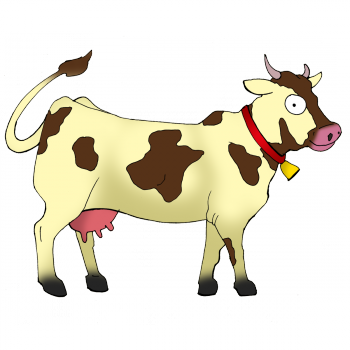
\includegraphics[keepaspectratio=true,height=0.6\textheight]{images/cow.png}
	\end{center}
\end{frame}

\begin{frame}{The Problem}
	\begin{center}
		In real life, we need to have \textbf{more pets} and \textbf{more milk} to exchange it for some \textbf{toys} 
	\end{center}
\end{frame}

\begin{frame}{The Problem}
	\begin{center}
		Building a farm is \textbf{hard} and \textbf{expensive} and caring about is \textbf{so time consuming} (:
		\end{center}
\end{frame}

\begin{frame}{The Idea}
	\begin{center}
		Let's use some \textbf{DevOps} magic
	\end{center}
\end{frame}

\begin{frame}{The Super Cow}
	\textbf{Instantly} in production, \textbf{no feeding}
	\begin{center}
		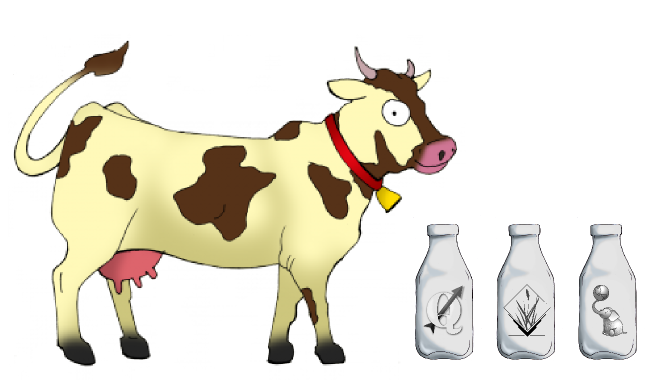
\includegraphics[keepaspectratio=true,height=0.6\textheight]{images/cow-geospatial.png}
	\end{center}
\end{frame}


\section{What is GIS.lab ?}
\begin{frame}
	\begin{center}
		\LARGE\textbf{What is GIS.lab ?}
	\end{center}
\end{frame}

\begin{frame}{What is GIS.lab ?}
	\textbf{Free} technology which can \textbf{instantly} turn any computer network in to the \textbf{fully equipped geospatial cluster}
	\begin{center}
		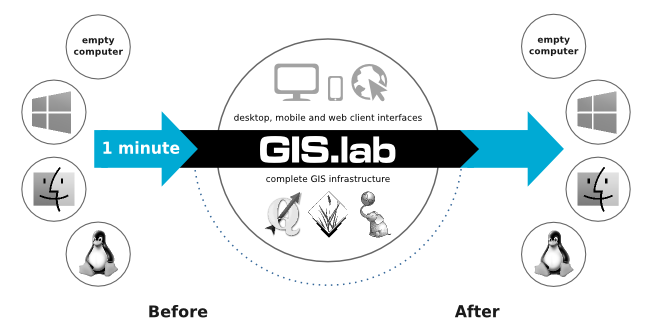
\includegraphics[keepaspectratio=true,height=0.5\textheight]{images/gislab-schema.png}
	\end{center}
\end{frame}

\begin{frame}{What is GIS.lab ?}
	\begin{center}
		and \textbf{back} again
	\end{center}
\end{frame}

\begin{frame}{Key Features}
	\begin{itemize}
		\item only \textbf{single one machine} needs to be installed per network
		\item fully \textbf{automatic} installation
		\item client machines are working \textbf{out-of-box}
		\item contains everything \textbf{from data storage} to \textbf{mobile client interface}
	\end{itemize}
\end{frame}

\begin{frame}{Key Features}
	\begin{itemize}[<+->]
		\item \textbf{instant} deployment
		\item \textbf{central management}
		\item \textbf{desktop, web and mobile} client interfaces
		\item automatic \textbf{clustering} and \textbf{computing power sharing}
		\item \textbf{no dependencies}
	\end{itemize}
\end{frame}

\begin{frame}{GIS.lab Cluster Architecture}
	\begin{center}
		
\includegraphics[keepaspectratio=true,height=0.8\textheight]{images/gislab-cluster-architecture.png}
	\end{center}
\end{frame}

\begin{frame}{GIS.lab Server (Master)}
%\	\begin{center}
%\		
\includegraphics[keepaspectratio=true,height=0.3\textheight]{images/image.png}
%\	\end{center}
	\begin{itemize}
		\item \textbf{cluster} orchestration
		\item \textbf{data storage} and \textbf{sharing}
		\item \textbf{load balancing}
	\end{itemize}
\end{frame}

\begin{frame}{GIS.lab Clients}
%\	\begin{center}
%\		
\includegraphics[keepaspectratio=true,height=0.3\textheight]{images/image.png}
%\	\end{center}
	\begin{itemize}
		\item initialized \textbf{from server}
		\item \textbf{user interfaces} for data processing, analysis and collaboration
		\item \textbf{computing power} for cluster
	\end{itemize}
\end{frame}

\begin{frame}{Desktop, Web and Mobile Client Interfaces}
	\begin{center}
		%\image: desktop + web + mobile schemas
		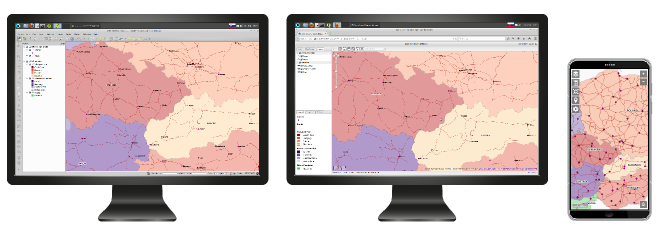
\includegraphics[keepaspectratio=true,height=0.5\textheight]{images/gislab-desktop-web-mobile.png}
	\end{center}
\end{frame}


\section{Deployment}
\begin{frame}
	\begin{center}
		\LARGE\textbf{Deployment}	
	\end{center}
\end{frame}

\begin{frame}{Automatic Installation}
	\begin{center}
		
\includegraphics[keepaspectratio=true,height=0.4\textheight]{images/ansible.png}
	\end{center}
	\begin{itemize}
		\item \textbf{human-readable} IT automation language
		\item \textbf{self-documenting} syntax
		\item \textbf{agent-less} execution
	\end{itemize}
\end{frame}

\begin{frame}{Automatic Installation}
	\begin{center}
		
\includegraphics[keepaspectratio=true,height=0.4\textheight]{images/ansible.png}
	\end{center}
	\begin{itemize}
		\item idempotent \textbf{modules, templates}
		\item support for \textbf{cloud providers} AWS, GCE, Digital Ocean, Azure ...
	\end{itemize}
\end{frame}

\begin{frame}[fragile]{Automatic Installation}
	\begin{center}
		
\includegraphics[keepaspectratio=true,height=0.4\textheight]{images/ansible.png}
	\end{center}

   \lstset{language=sh}
	\begin{lstlisting}
		$ ansible-playbook
		  --inventory=gislab.inventory
		  --private-key=~/.ssh/id_rsa
		  system/gislab.yml
	\end{lstlisting}
\end{frame}

\begin{frame}[fragile]{Virtual Machine - Development and Testing}
	\begin{center}
		
\includegraphics[keepaspectratio=true,height=0.35\textheight]{images/vagrant.png}
		
\includegraphics[keepaspectratio=true,height=0.35\textheight]{images/virtualbox.png}
		
\includegraphics[keepaspectratio=true,height=0.35\textheight]{images/ansible.png}
	\end{center}

   \lstset{language=sh}
	\begin{lstlisting}
		$ vagrant up

		Bringing machine 'gislab_vagrant' up with 'virtualbox' provider...
		==> gislab_vagrant: Importing base box 'precise-canonical'...
		==> gislab_vagrant: Running provisioner: install (ansible)...
	\end{lstlisting}
\end{frame}

\begin{frame}{GIS.lab Unit - End User Deployment}
	\begin{center}
		
\includegraphics[keepaspectratio=true,height=0.5\textheight]{images/gislab-unit.png}
	\end{center}
	\begin{itemize}
		\item Intel Haswell, \textbf{16 GB RAM}, \textbf{SSD}, tested with \textbf{20 clients}
		\item \textbf{portable}, \textbf{pocket size} (11 x 11 x 4 cm)
		\item \textbf{plug-and-play}
		\item \textbf{automatic} host \textbf{network adaptation}
	\end{itemize}
\end{frame}


\section{Client Interfaces}
\begin{frame}
	\begin{center}
		\LARGE\textbf{Client Interfaces}
	\end{center}
\end{frame}

\begin{frame}[plain]{Client Interfaces Architecture}
	\begin{center}
		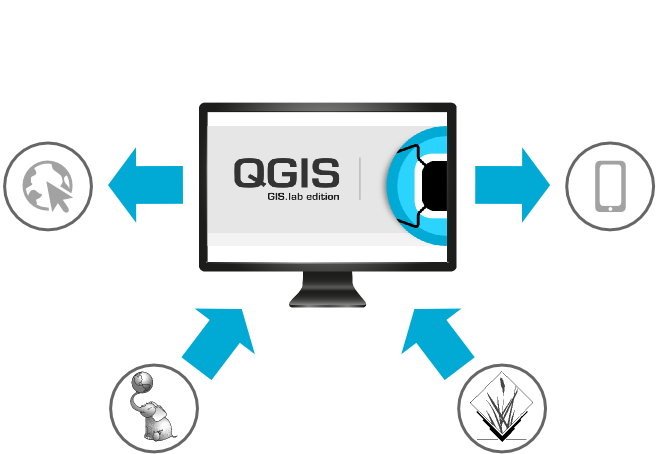
\includegraphics[keepaspectratio=true,width=\textwidth]{images/gislab-client-interfaces.png}
	\end{center}
\end{frame}

\begin{frame}[plain]{Publishing to Web and Mobile}
	\begin{center}
		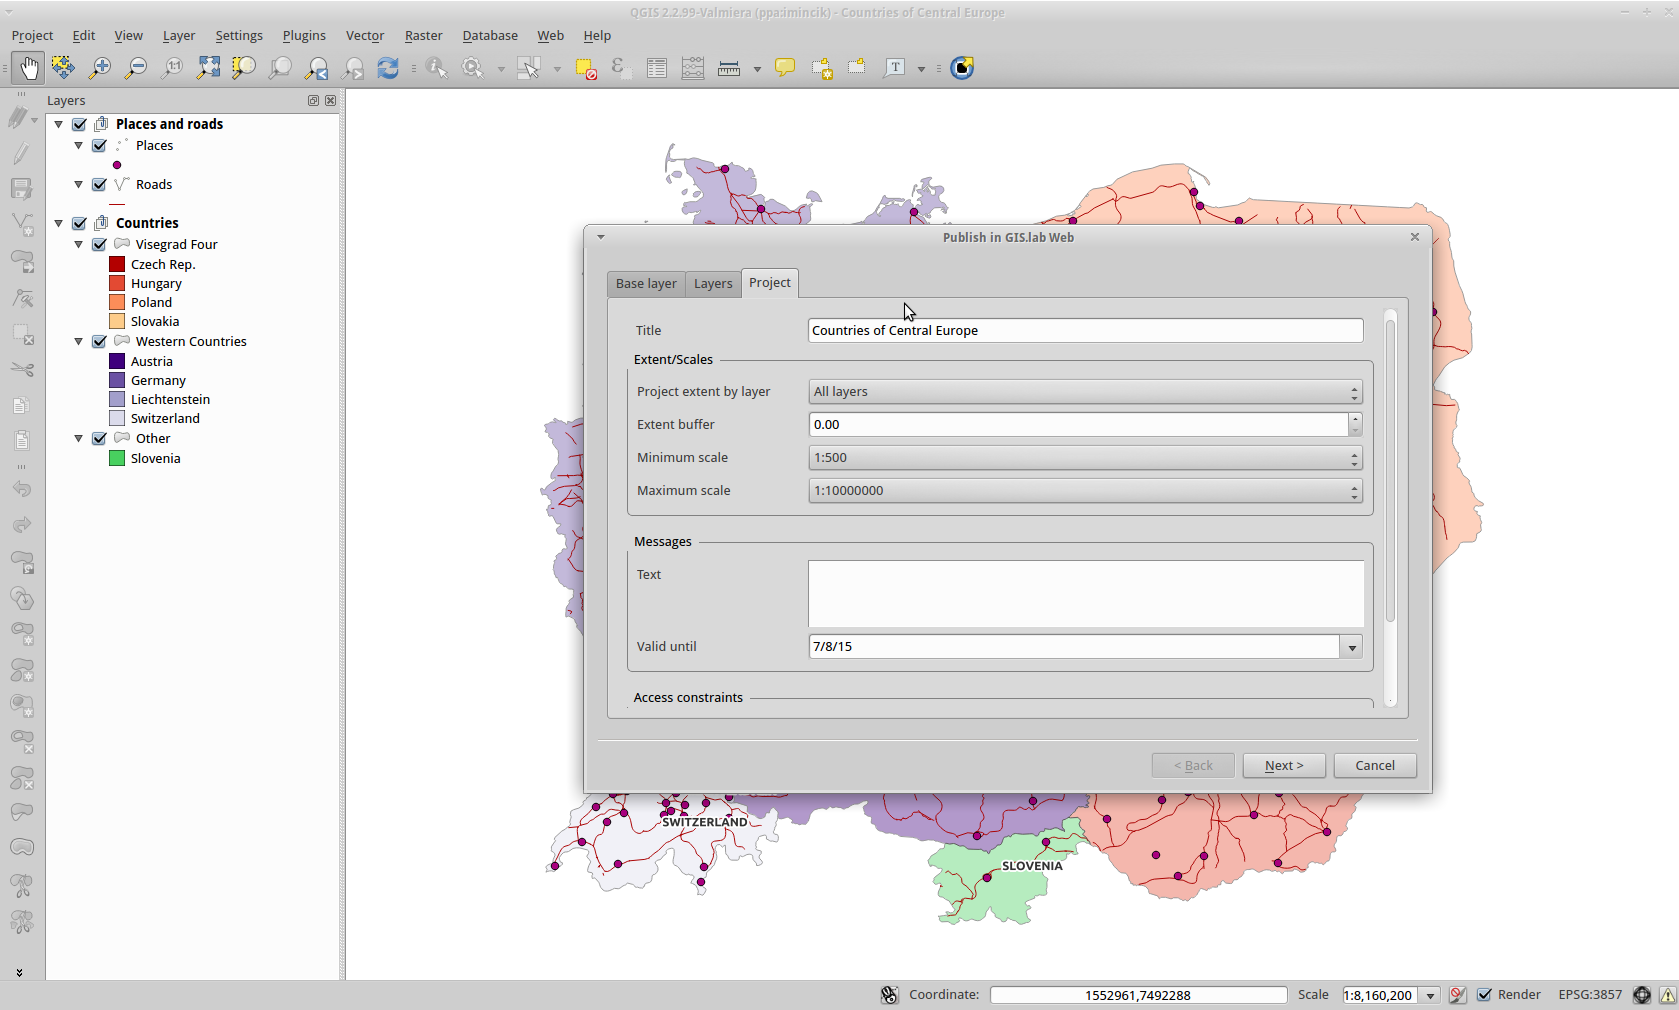
\includegraphics[keepaspectratio=true,width=\textwidth]{images/gislab-publish.png}
	\end{center}
\end{frame}


\begin{frame}
	\begin{center}
		\LARGE\textbf{Desktop}	
	\end{center}
\end{frame}

\begin{frame}{Desktop Interface}
	\begin{center}
		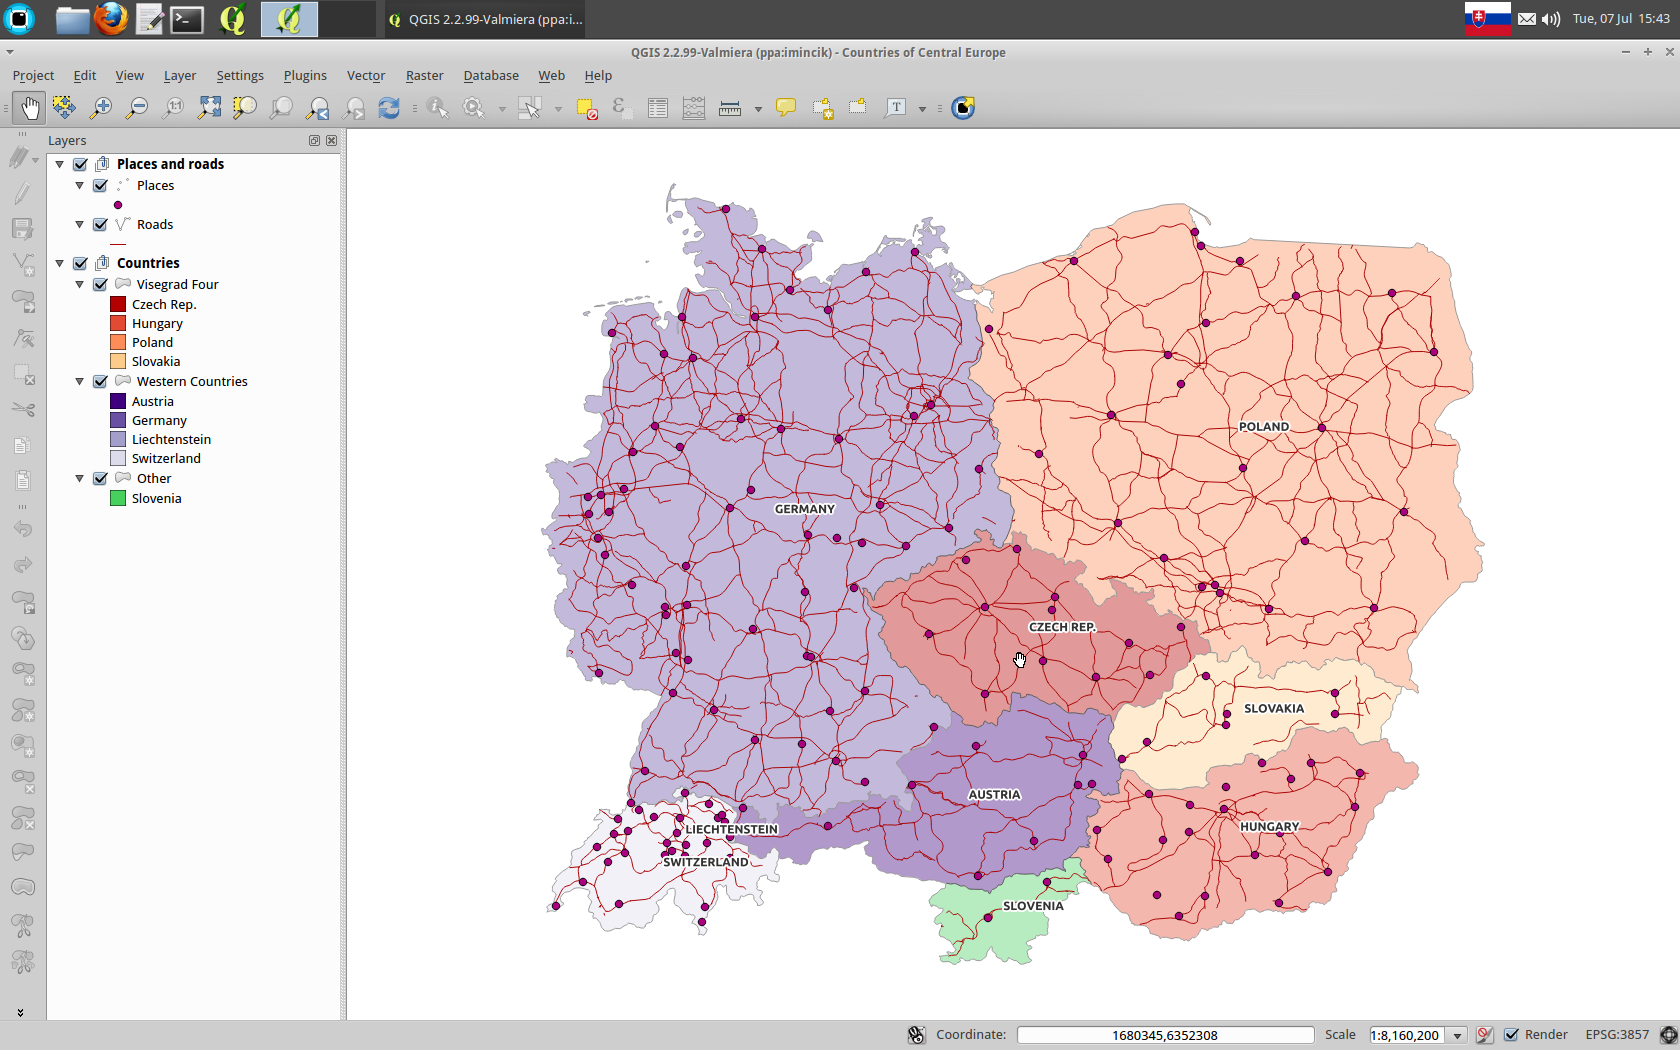
\includegraphics[keepaspectratio=true,height=0.5\textheight]{images/gislab-desktop.png}
	\end{center}
	\begin{itemize}
		\item \textbf{traditional}, \textbf{customized}, \textbf{low resources} environment
		\item \textbf{office} and \textbf{geospatial} software
		\item combination of \textbf{desktop performance} with \textbf{web accessibility}
	\end{itemize}
\end{frame}

\begin{frame}[plain]{Desktop Interface}
	\begin{center}
		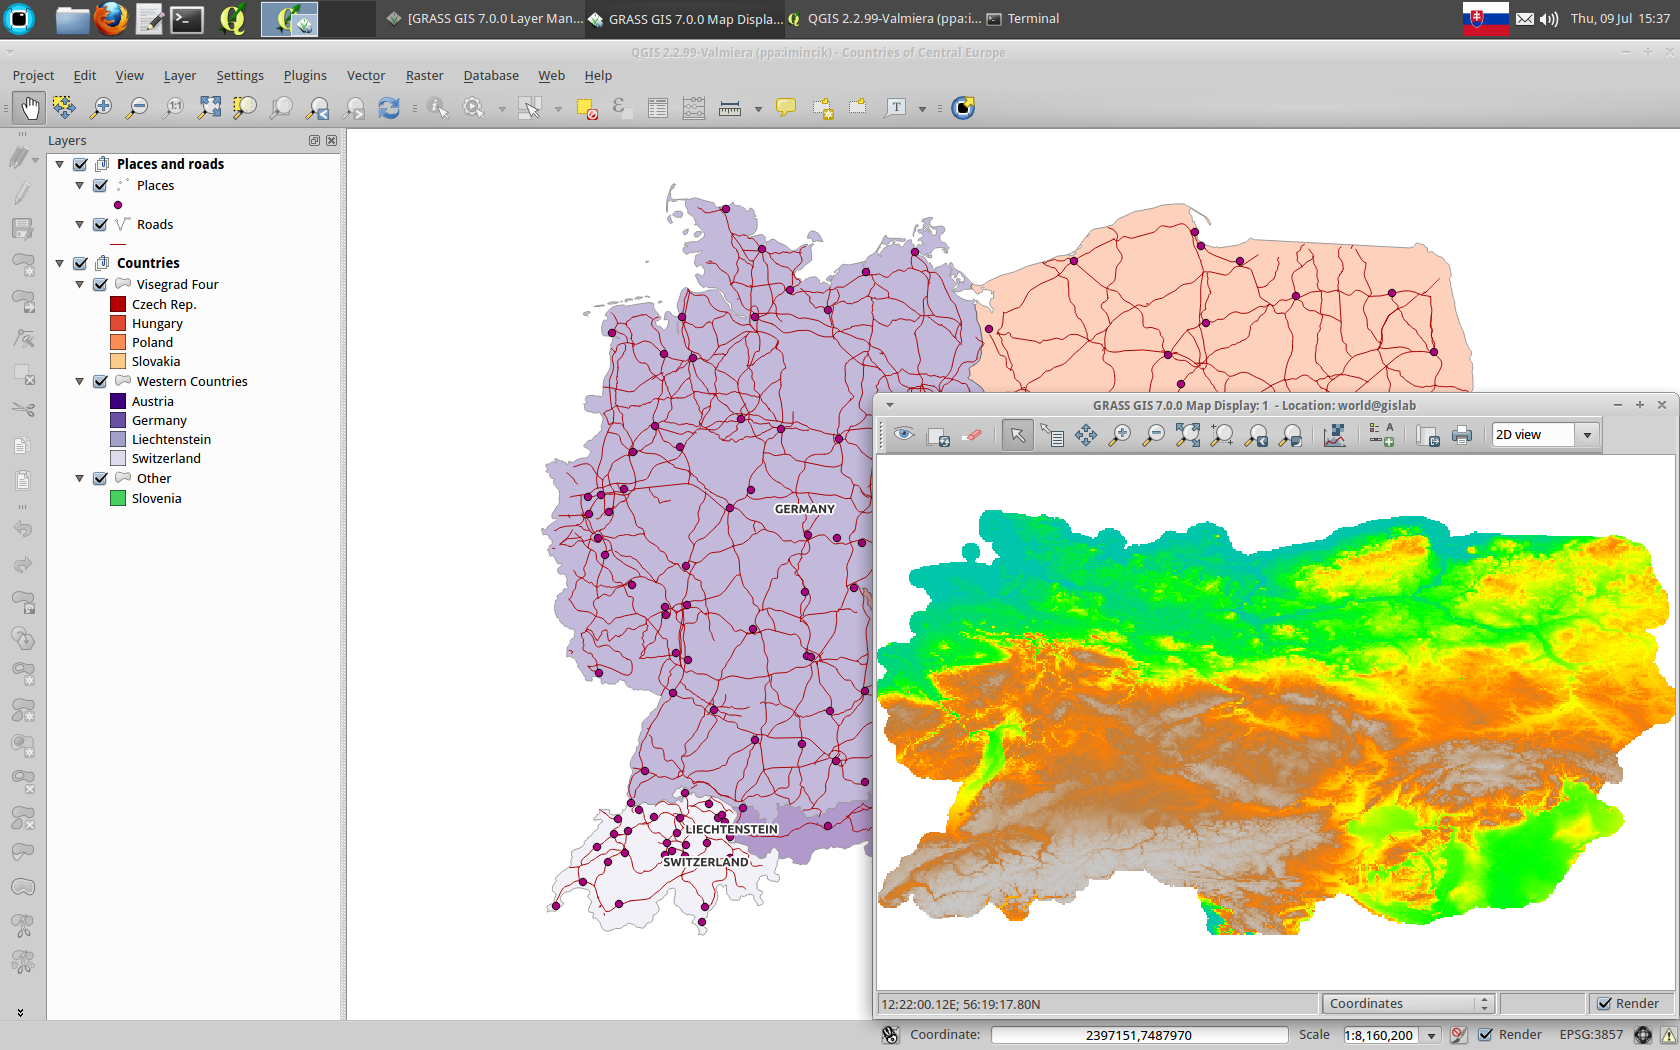
\includegraphics[keepaspectratio=true,width=\textwidth]{images/gislab-desktop-2.png}
	\end{center}
\end{frame}

\begin{frame}{Machines Initialization}
	\begin{center}
		%\ image: boot from server
		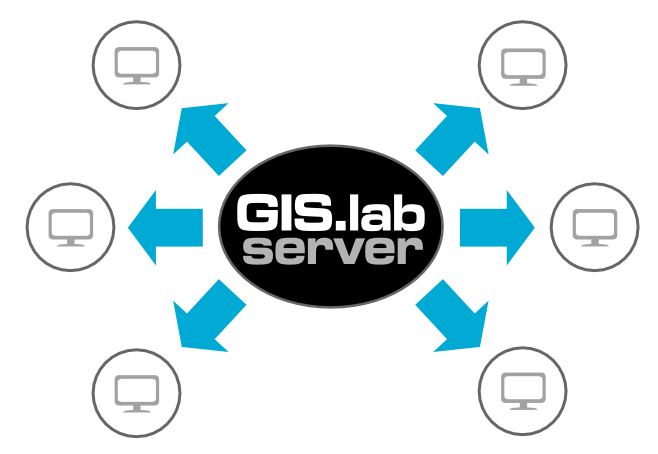
\includegraphics[keepaspectratio=true,height=0.4\textheight]{images/gislab-machines-launch.png}
	\end{center}
	\begin{itemize}
		\item \textbf{initialized} from \textbf{GIS.lab network} (PXE, HTTP)
		\item always \textbf{clean system}, \textbf{maintenance-free}
		\item \textbf{no HDD} required
		\item using \textbf{full hardware potential} - opposite to thin client
	\end{itemize}
\end{frame}

\begin{frame}{Physical or Virtual Mode}
	\begin{center}
		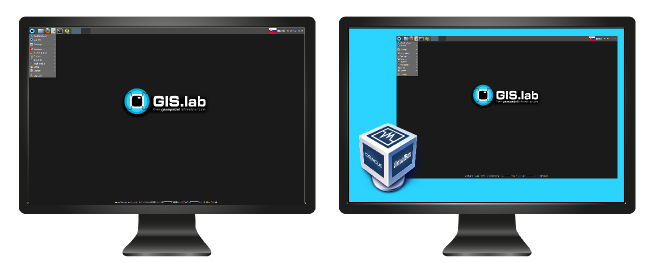
\includegraphics[keepaspectratio=true,height=0.5\textheight]{images/physical-or-virtual-mode.png}
	\end{center}
	\begin{itemize}
		\item \textbf{physical mode}: best performance, original OS is temporary lost
		\item \textbf{virtual mode}: any OS, original OS and GIS.lab are available
	\end{itemize}
\end{frame}

\begin{frame}[fragile]{Customization}
	\lstset{language=sh}
	\begin{lstlisting}
		$ gislab-client-shell -i   # enter client env

		$ apt-get install gedit    # install Gedit
		$ exit                     # exit client env

		$ gislab-client-image      # deploy updated client image
	\end{lstlisting}

	\begin{itemize}
		\item \textbf{well known} tools
		\item \textbf{rollback}
	\end{itemize}
\end{frame}

\begin{frame}[fragile]{Booster File System}
	\textbf{Test writing of 2 GB file}
	\\
	HDD
	\lstset{language=sh}
	\begin{lstlisting}
		$ dd if=/dev/zero of=/tmp/test.f bs=1M count=2048
		  2147483648 bytes (2,1 GB) copied, 24,8055 s, 86,6 MB/s
	\end{lstlisting}

	Booster
	\lstset{language=sh}
	\begin{lstlisting}
		$ dd if=/dev/zero of=~/Booster/test.f bs=1M count=2048
		  2147483648 bytes (2,1 GB) copied, 0,582147 s, 3,7 GB/s
	\end{lstlisting}

	\begin{itemize}
		\item \textbf{super fast} file system in RAM
		\item ideal for \textbf{temporary files}
	\end{itemize}
\end{frame}

\begin{frame}
	\begin{center}
		\LARGE\textbf{Web and Mobile}
	\end{center}
\end{frame}

\begin{frame}{Web and Mobile Interface}
	\begin{center}
		%\ image: web and mobile client screenshots
		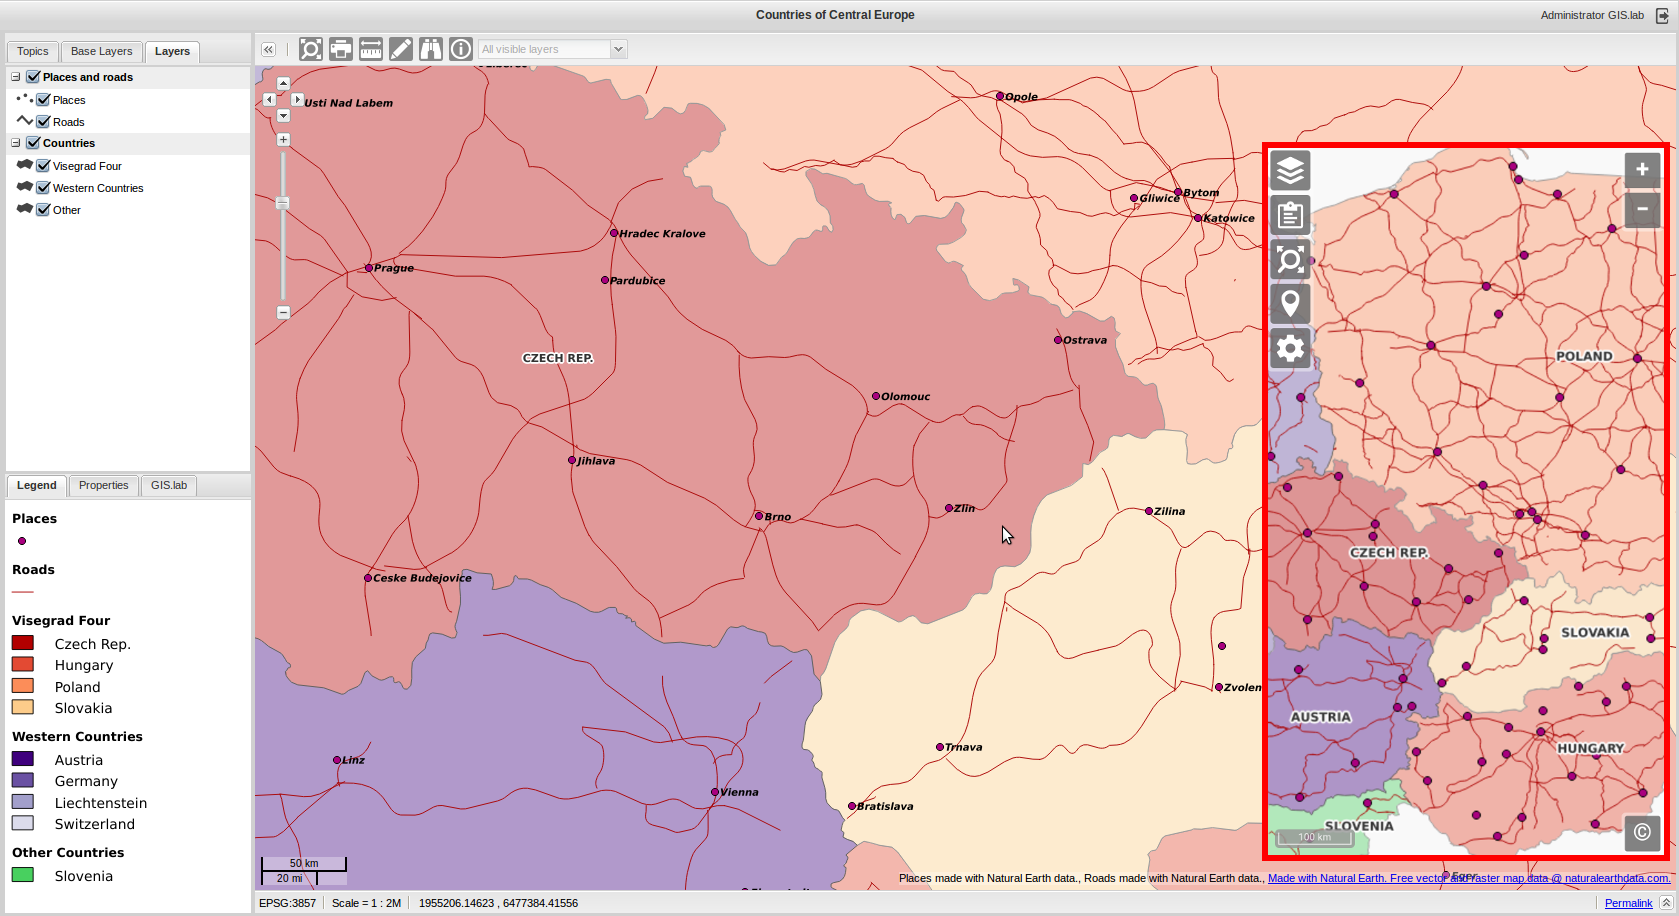
\includegraphics[keepaspectratio=true,height=0.5\textheight]{images/gislab-web+mobile.png}
	\end{center}
	\begin{itemize}
		\item \textbf{themes}, \textbf{base} and \textbf{overlay} layers
		\item advanced \textbf{search} forms
		\item \textbf{print} outputs
		\item vector features \textbf{drawing} and \textbf{sharing}
	\end{itemize}
\end{frame}

\begin{frame}[plain]{Web Interface}
	\begin{center}
		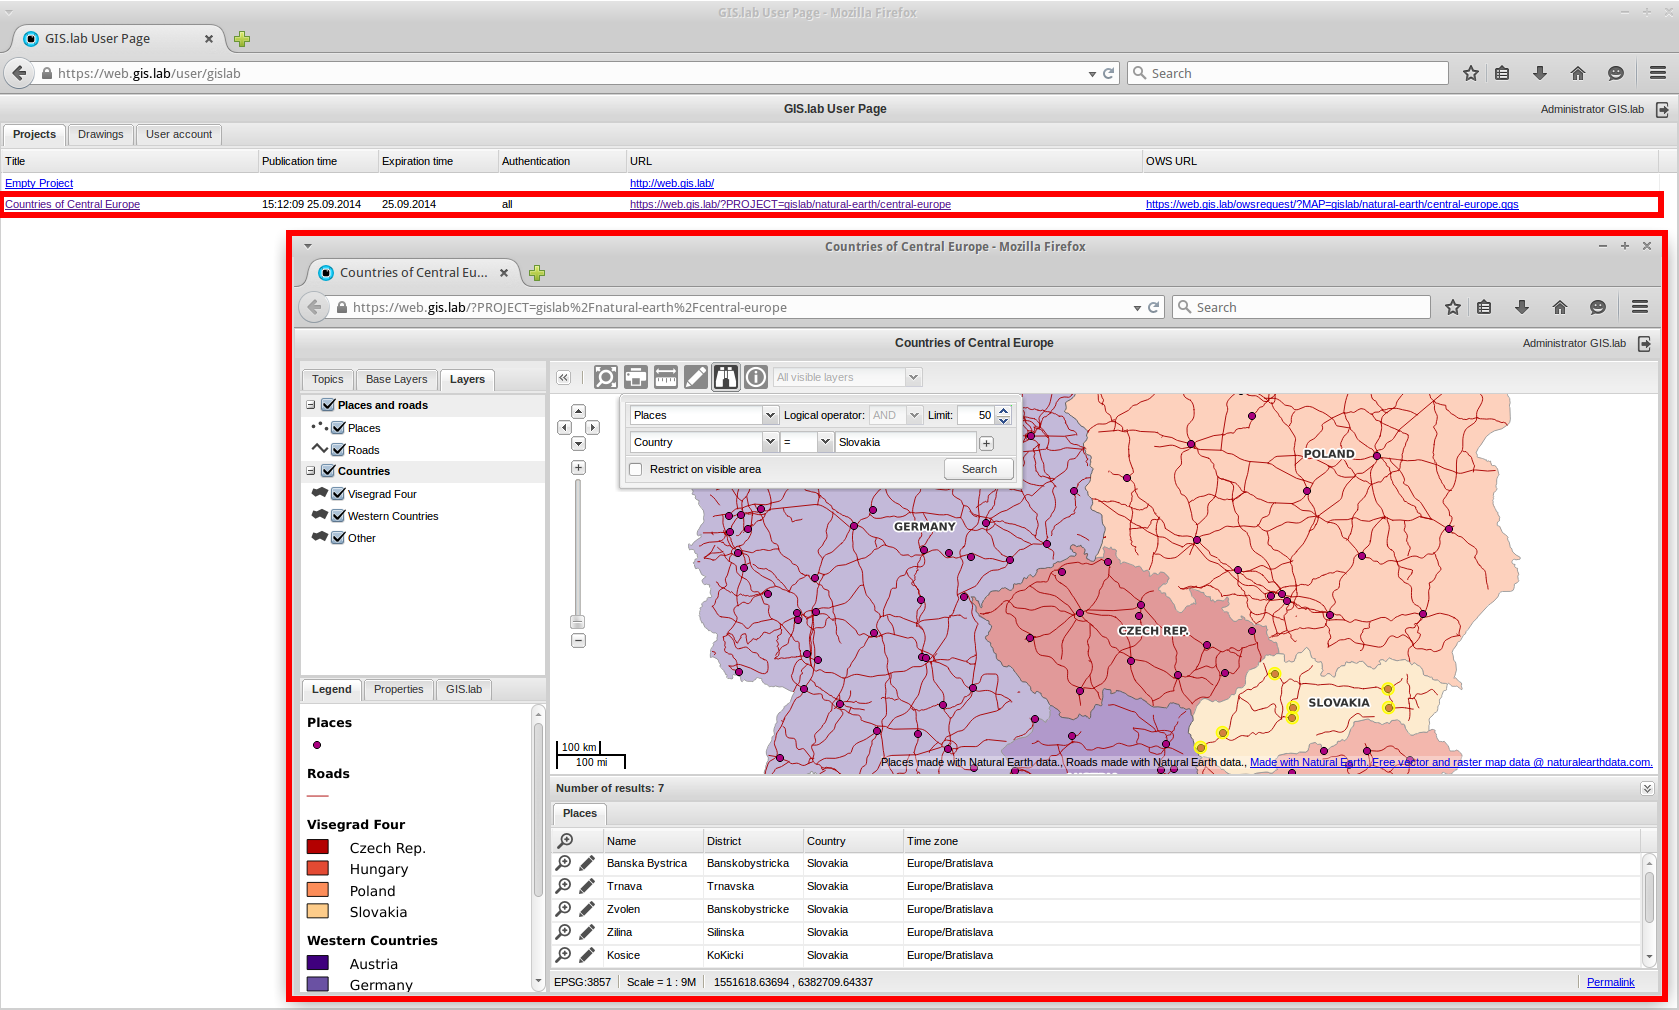
\includegraphics[keepaspectratio=true,width=\textwidth]{images/gislab-web-2.png}
	\end{center}
\end{frame}

\begin{frame}[plain]{Mobile Interface}
	\begin{center}
		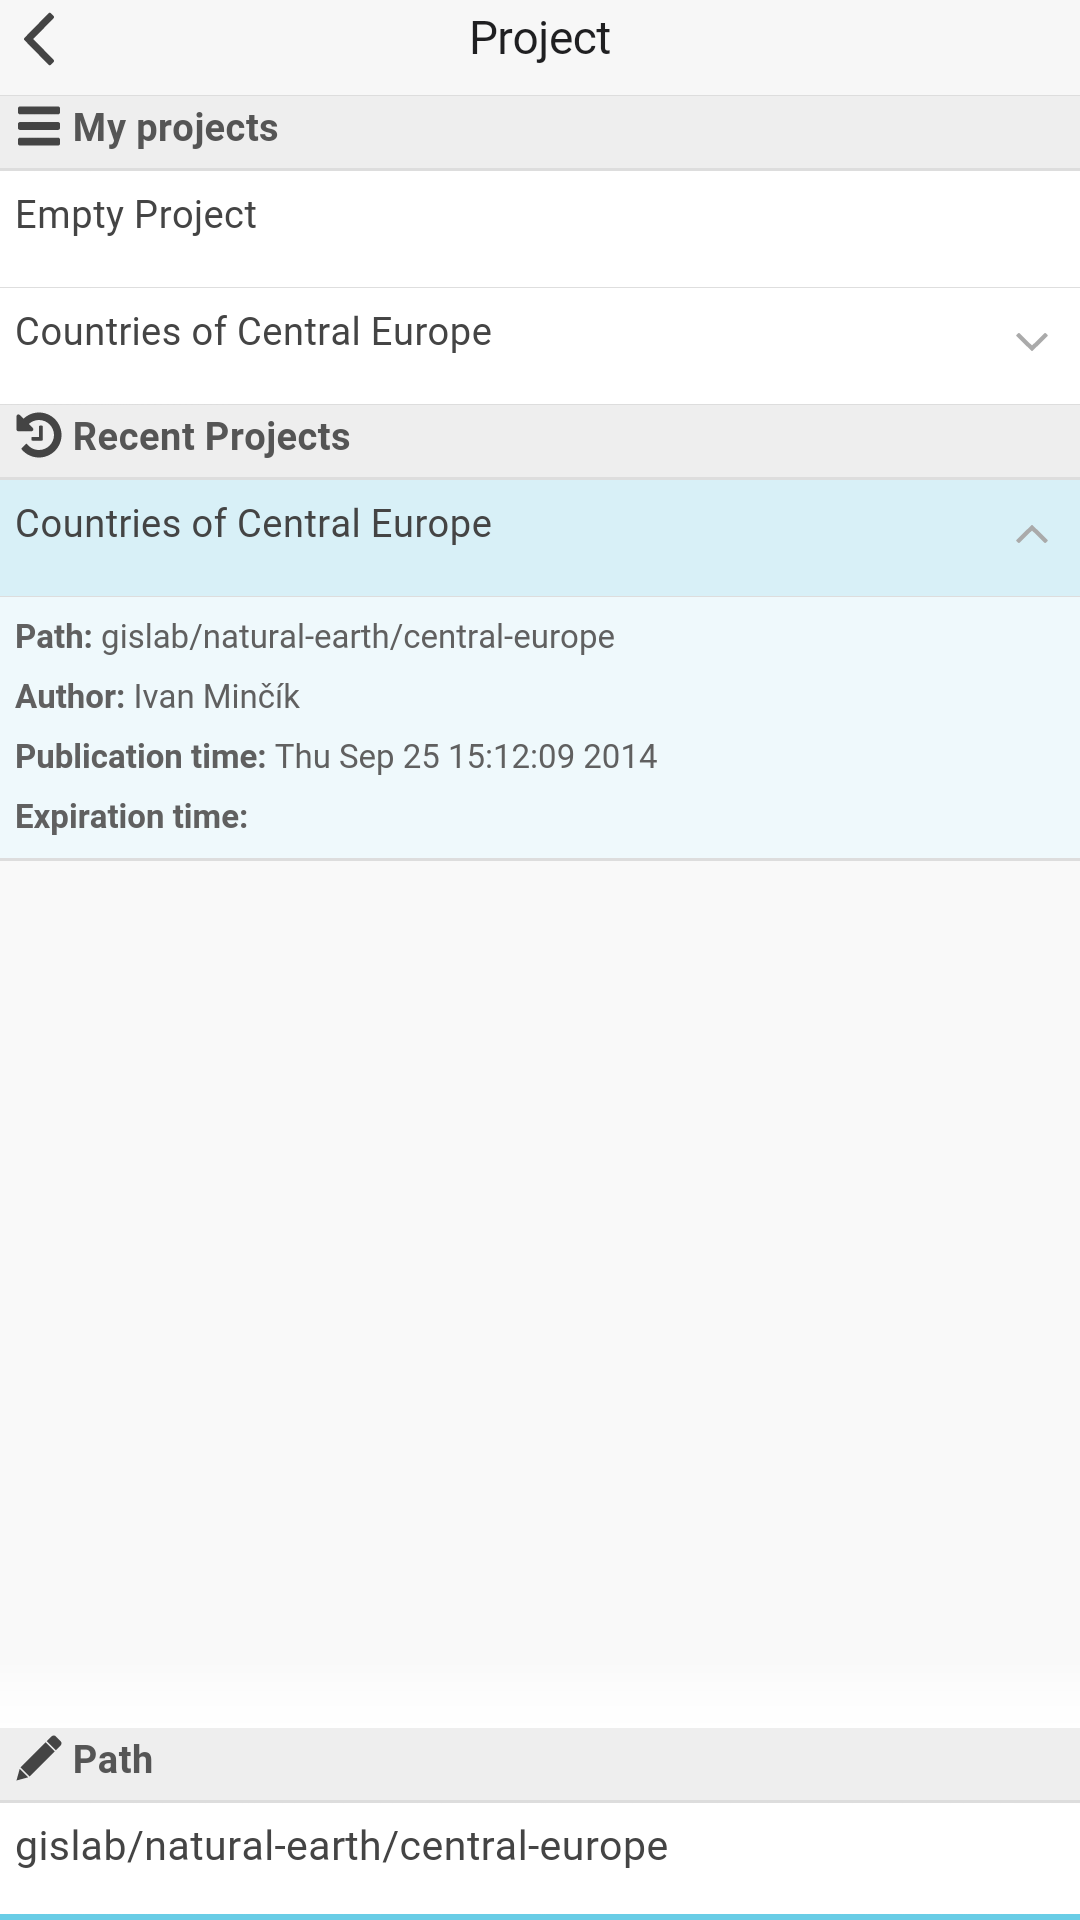
\includegraphics[keepaspectratio=true,width=0.4\textwidth]{images/gislab-mobile.png}\hspace*{0.5cm}
		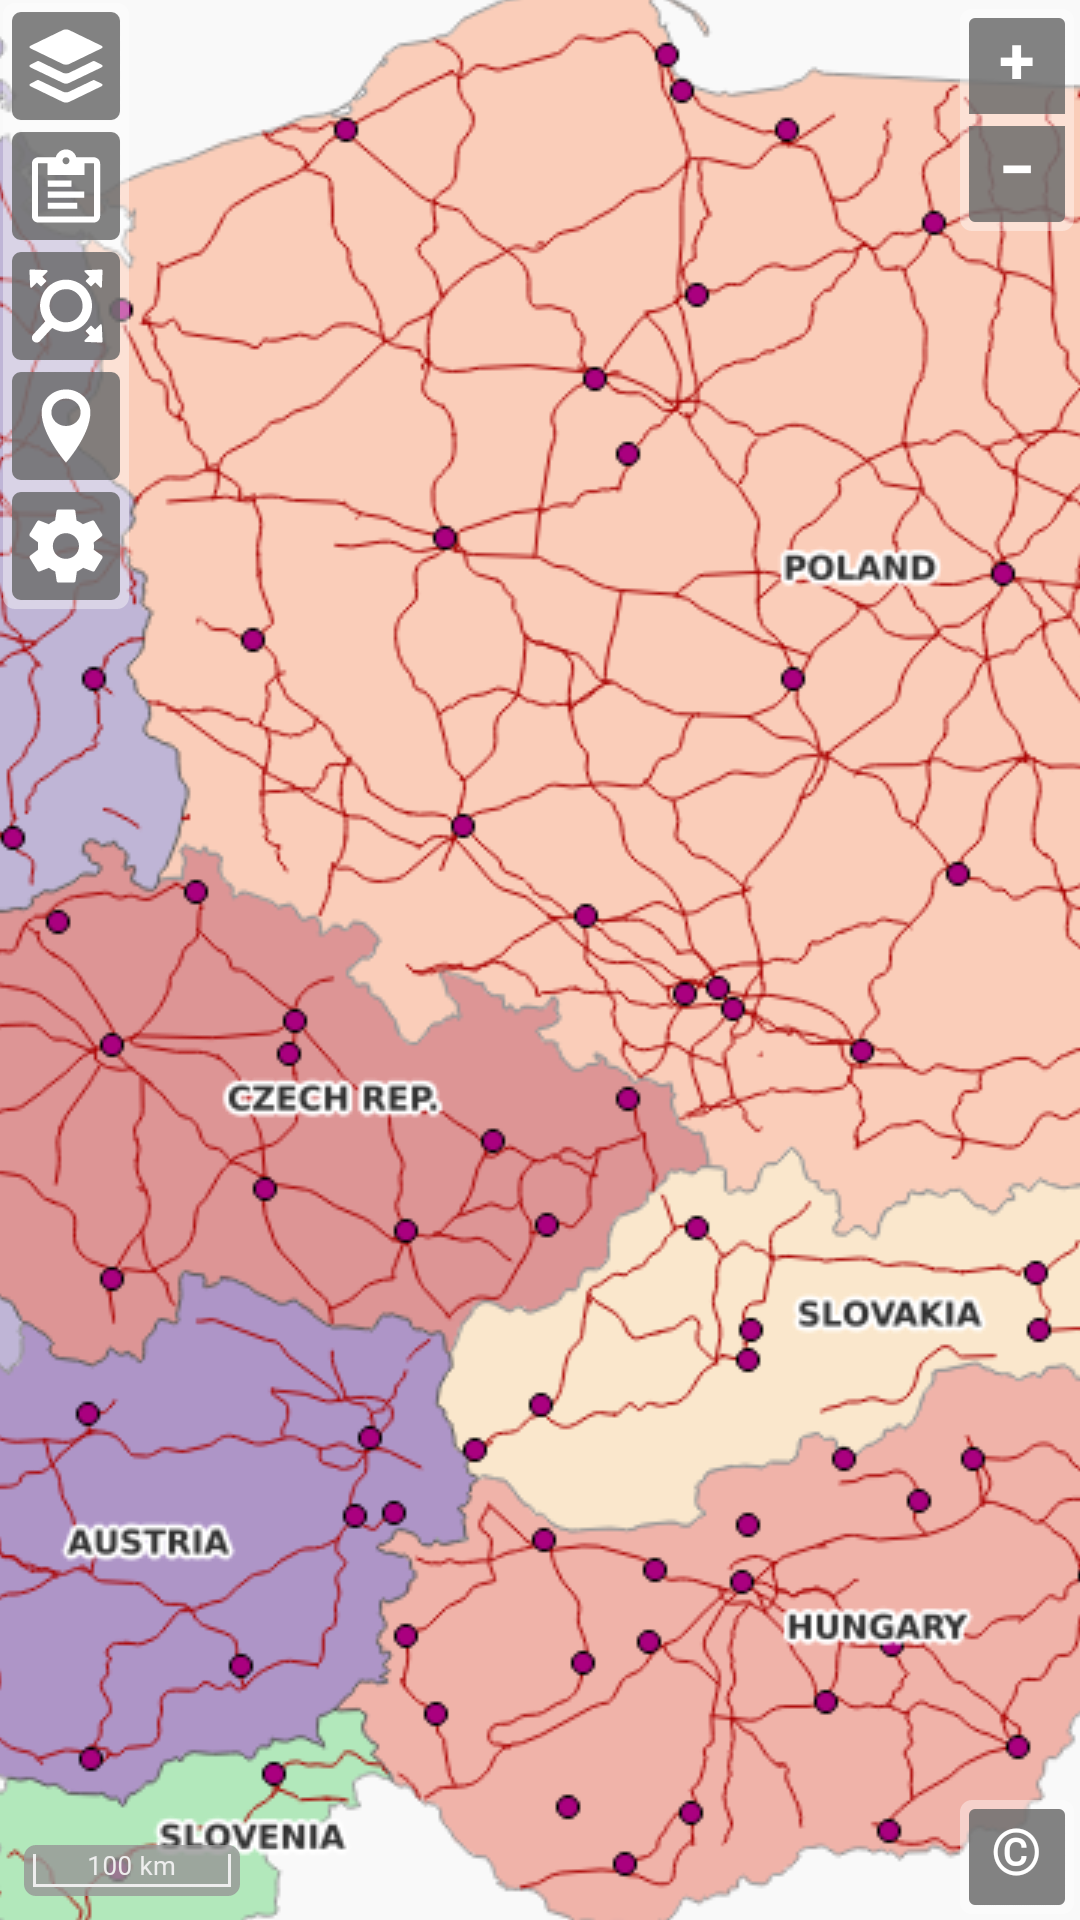
\includegraphics[keepaspectratio=true,width=0.4\textwidth]{images/gislab-mobile-3.png}
	\end{center}
\end{frame}


\section{Cluster}
\begin{frame}
	\begin{center}
		\LARGE\textbf{Cluster}	
	\end{center}
\end{frame}

\begin{frame}{Automatic Cluster Orchestration}
	\begin{center}
		
\includegraphics[keepaspectratio=true,height=0.5\textheight]{images/serf.png}
	\end{center}
	\begin{itemize}
		\item \textbf{server} and \textbf{client machines}
		\item \textbf{decentralized} cluster \textbf{membership} and \textbf{failure detection} system based on GOSSIP protocol
	\end{itemize}
\end{frame}

\begin{frame}[fragile]{Basic Information About Machines}
	\lstset{language=sh}
	\begin{lstlisting}
		$ gislab-cluster members					# format text or json 

		server.gis.lab  192.168.15.5:7946 
		                alive  role=server

		c50             192.168.15.50:7946
		                alive
		                role=client,worker=yes,session-active=user1

		c51             192.168.15.51:7946
		                left
		                role=client,worker=yes
	\end{lstlisting}
\end{frame}

\begin{frame}[fragile]{Events and Queries}
	\textbf{Syntax}
	\lstset{language=sh}
	\begin{lstlisting}
		$ gislab-cluster event <EVENT-NAME>
		$ gislab-cluster query <QUERY-NAME>		
	\end{lstlisting}

	\textbf{Reboot event}
	\lstset{language=sh}
	\begin{lstlisting}
		$ gislab-cluster event reboot
	\end{lstlisting}
\end{frame}

\begin{frame}[fragile]{Parallel Commands Execution}
	\textbf{Detection of running (alive) client machines}
	\lstset{language=sh}
	\begin{lstlisting}
		$ MACHINES="$(gislab-cluster members
			  -status=alive
			  -tag role=client ...
		)"
	\end{lstlisting}
	
	\textbf{Parallel installation of Gedit package}
	\begin{lstlisting}
		$ parallel-ssh -H "$MACHINES"

		  sudo DEBIAN_FRONTEND=noninteractive
		  apt-get install -y --no-install-recommends gedit
		  
		  ...
		  [1] 23:02:57 [SUCCESS] c51
		  [1] 23:02:57 [SUCCESS] c51
		  ...
	\end{lstlisting}
\end{frame}

\begin{frame}[fragile]{Stronger With Each Client Machine}
	\textbf{OWS load balancing}

	\lstset{language=sh}
	\begin{lstlisting}
		$ while true; do
		    curl "http://ms.gis.lab:90/cgi-bin/qgis_mapserv?
		      SERVICE=WMS&REQUEST=GetCapabilities"
		  done
	\end{lstlisting}
	\begin{center}
		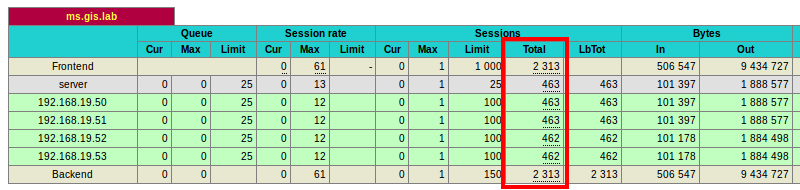
\includegraphics[keepaspectratio=true,width=\textwidth]{images/lb-stats.png}
	\end{center}
\end{frame}

\section{Other}
\begin{frame}
	\begin{center}
		\LARGE\textbf{Other}
	\end{center}
\end{frame}

\begin{frame}[fragile]{Integration Test Suite}
	\lstset{language=sh}
	\begin{lstlisting}
		$ vagrant provision --provision-with test
		...
		TASK: [basic-server-configuration-test | Test if ordinary test user account exists in PostgreSQL]
		...
		TASK: [service-dns-test | Test 'gis.lab' DNS records are resolved]
		...
		TASK: [service-mapserver-test | Test WMS GetCapabilies request with example GIS.lab project]
		...
		TASK: [service-mapserver-test | Test WMS GetMap request with example GIS.lab project]
		...
	\end{lstlisting}
\end{frame}

\begin{frame}{Where to Use ?}
	\begin{itemize}
		\item \textbf{schools}: central management, maintenance-free clients
		\item \textbf{science}: horizontally scalable computing power, advanced tools, extensibility
		\item \textbf{small projects}: affordable, complete solution
		\item \textbf{poor countries}: low system requirements, maintenance-free clients
		\item \textbf{crisis management}: portable, instant deployment, no dependencies
	\end{itemize}
\end{frame}

\begin{frame}{Future Plans}
	\begin{itemize}
		\item \textbf{web administration} interface
		\item integration of \textbf{GRASS WPS} services
		\item integration of \textbf{data science} tools
		\item \textbf{web client} rewrite with \textbf{OL 3}
		\item update to \textbf{Ubuntu 16.04} and \textbf{systemd}
	\end{itemize}
\end{frame}

\begin{frame}[plain]{Good Night And Don't Worry About Pets}
	\begin{center}
		
\includegraphics[keepaspectratio=true,width=\textwidth]{images/fairy-tail/dedusko-vecernicek.jpg}
	\end{center}
\end{frame}

\begin{frame}[plain]
	\begin{center}
		\textbf{http://web.gislab.io}\\
		\textbf{wiki:Quick-Start}\\
		\textbf{gis.lab@lists.osgeo.org}
	\end{center}
\end{frame}


% document END
\end{document}